\chapter{Mission: Cyber}

\emph{\emph{Cyber} is a RECON+ mission played on a~2'x3' play area.}


\section{Play Area}
\vspace{-2\parskip}
\noindent\begin{stdminipage}{\linewidth-(2in+1.5em)}
\vspace{0pt}   
\noindent
The Deployment Zones are~6'' areas along the short
play area edges.

Four Consoles are placed in a grid, each~6'' from a long edge of the
play area and~8'' from a deployment zone.

A Network Terminal is placed at the center of the play area.

\section{Mission Rules}

The Connect Objective short skill may be applied to Consoles in this
mission.  The Consoles are Repeaters for the Hackers of both players.
They do not apply Firewall MODs.

\end{stdminipage}
\hfill
\begin{minipage}[t]{2in}\centering
\vspace{4pt}   
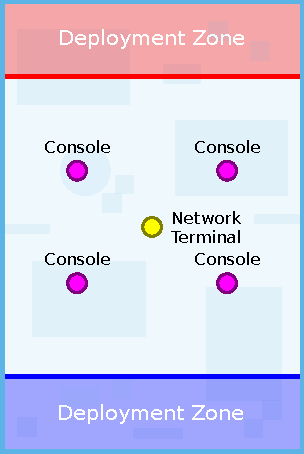
\includegraphics{maps/map-cyber}
\end{minipage}

\section{Scoring}

Players may score up to~10 objective points via the following
conditions at game end:
\begin{itemize}\shortlist
\item 1pt for each Console closest to your Deployment Zone connected.
\item 2pts for each Console farthest from your Deployment Zone
  connected.
\item 2pts for having your Special Agent in base contact with a
  connected Console.
\item 1pt if more points of the opposing army list have been destroyed.
\item 1pt if the opposing Special Agent is in a Null state or eliminated.
\end{itemize}

\vfill
\vbox to 0pt{}